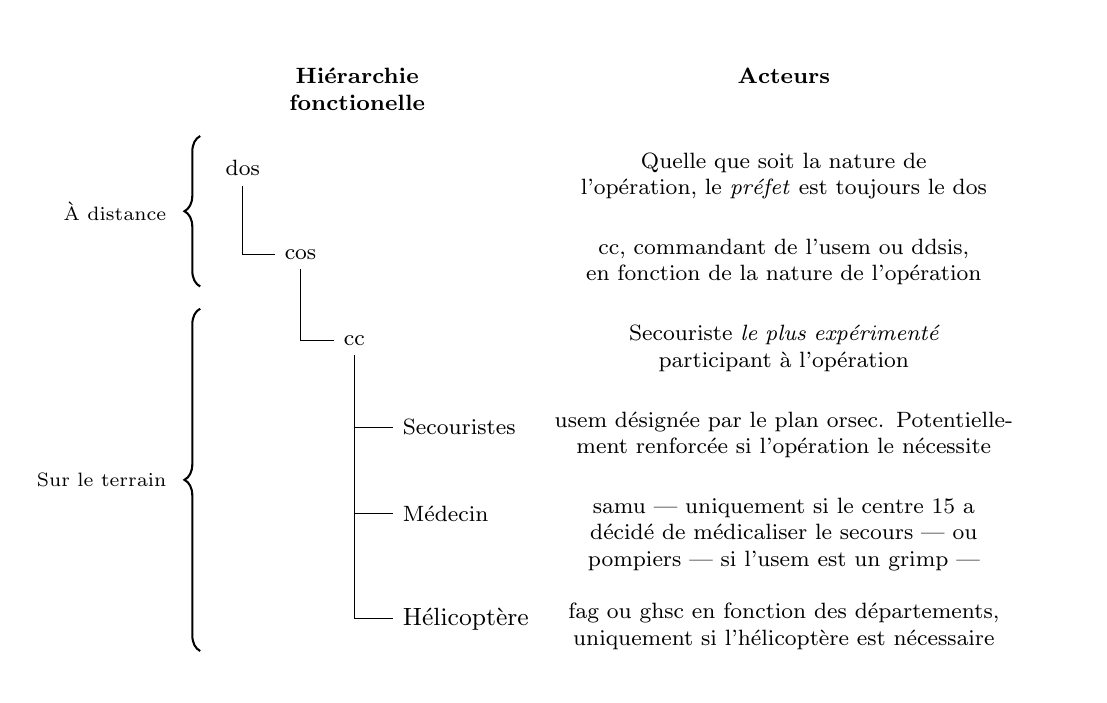
\begin{tikzpicture}
\usetikzlibrary{matrix, fit}
\usetikzlibrary{decorations.pathreplacing, calc}

\tikzset{ 
table/.style={
  matrix of nodes,
  nodes={align=center, font=\footnotesize,  minimum height=10mm},
  nodes in empty cells,
  column 1/.style={nodes={text width=9.5em}},
  column 2/.style={nodes={text width=20em}}
  }
}

\matrix (m) [table] {
    \toprule
  {\bfseries Hiérarchie fonctionelle} & {\bfseries Acteurs} \\
\midrule
   & Quelle que soit la nature de l'opération, le \emph{préfet} est
   toujours le dos\\
   & \ac{cc}, commandant de l'\ac{usem} ou \ac{ddsis}, en fonction de
   la nature de l'opération\\
&Secouriste \emph{le plus expérimenté} participant à l'opération\\
    &\ac{usem} désignée par le  plan \ac{orsec}. Potentiellement renforcée si l'opération le nécessite\\
    &\ac{samu} ---~uniquement si le centre 15 a décidé de médicaliser
    le secours~--- ou pompiers ---~si l'\ac{usem} est un \ac{grimp}~---\\
    &\ac{fag} ou \ac{ghsc} en fonction des départements, uniquement si l'hélicoptère est nécessaire\\};




\node[anchor=west](dos) at (m-2-1.west) {\footnotesize\ac{dos}};
\node[anchor=west](cos) at ([xshift=.75cm]m-3-1.west) {\footnotesize
  \ac{cos}};
\node[anchor=west](cc) at ([xshift=1.5cm]m-4-1.west) {\footnotesize\ac{cc}};
\node[anchor=west](sec) at ([xshift=2.25cm]m-5-1.west) {\footnotesize Secouristes};
\node[anchor=west](med) at ([xshift=2.25cm]m-6-1.west) {\footnotesize Médecin};
\node[anchor=west](heli) at ([xshift=2.25cm]m-7-1.west) {
  \small Hélicoptère};

\path[draw] (dos) |- (cos);
\path[draw] (cos) |- (cc);
\path[draw] (cc) |- (sec);
\path[draw] (cc) |- (med);
\path[draw] (cc) |- (heli);

		\draw [decorate,decoration={brace,amplitude=.2cm, raise=.2cm,mirror},line width=.75pt]  ([yshift=-.1cm]m-2-1.north west) -- ([yshift=.1cm]m-3-1.south west) node[midway, left, xshift=-.5cm]  {\scriptsize À distance};

		\draw [decorate,decoration={brace,amplitude=.2cm,
                  raise=.2cm,mirror},line width=.75pt]
                ([yshift=-.1cm]m-4-1.north west) --
                ([yshift=.1cm]m-7-1.south west) node[midway, left,
                xshift=-.5cm]  {\scriptsize Sur le terrain};
\end{tikzpicture}